\chapter{拓扑晶体绝缘体LaSbTe的层构造}\label{chap:lasbte}



\section{背景}
拓扑晶体绝缘体~\citep{fu2011topological}是由时间反演对称性保护的拓扑绝缘体~\citep{TIreview,qi2011,weng2015quantum}之外的一种由晶体对称性保护的拓扑态。由晶体平移对称性保护的三维弱拓扑绝缘体可以通过在第三个方向堆叠二维拓扑绝缘体得到。受此启发,除了平移对称性之外,由镜面对称性保护的拓扑晶体绝缘体也已经被发现可以绝热地连接到弱耦合的二维拓扑态极限,而这些二维的拓扑态可以是由镜面对称性保护的拓扑晶体绝缘体~\citep{kim2015},也可以是二维拓扑绝缘体~\citep{Fulga2016}。这些发现启发研究者们基于“降维理论”研究拓扑晶体绝缘体,现在称之为“层构造(LC)”方法。已经证明,所有的由晶体点群对称性保护的拓扑态都可以通过堆叠更低维度的拓扑态来获得,而且因此得到的拓扑分类既可以应用于相互作用的玻色子,也可以应用于自由费米子~\citep{huang2017,hsong2017,Songreal,Song2019}。通过这种方法,可以清晰地理解晶体对称性保护的拓扑态的物理本质。

我们所的方辰老师团队非常详细地利用了层构造方法,他们在存在时间反演对称性的情况下,推导出了从对称数据到任意空间群的拓扑不变量之间详尽的映射关系~\citep{song2017}。当与拓扑量子化学和对称性指标~\citep{tqc2017,nc_ashvin,Kruthoff2017}相结合时,这种映射关系提供了非常有效的方法来定义和搜索新的拓扑晶体绝缘体。层构造方法是用具有不平庸的$\mathbb{Z_2}$或者镜面陈数的二维绝缘体来搭建晶格,而原子绝缘体是由放在Wyckoff位置上合适的原子轨道组成。然而,层构造和所形成的拓扑晶体绝缘体之间的对应关系不像原子绝缘体的物理图像那么清晰。最近,Matsugatani和Watanabe使用紧束缚模型将高阶拓扑绝缘体与低维的拓扑态相联系,来展现高阶拓扑绝缘体的物理本质~\citep{haruki2018}。但是,目前还没有一个能够将实空间的低维拓扑态和动量空间能带拓扑之间精确的一对一关系展现出来的、实际的层状拓扑晶体绝缘体材料。

在我们的工作中,我们介绍了一个实际材料LaSbTe,这个材料有两个相:四方相($\tlasbte$)和正交相($\olasbte$),其中$\tlasbte$是$WHM$($W$ = Zr,Hf或La,$H$ =Si,Ge,Sn,或Sb,和$M$ = O,S,Se,或Te)家族的一员~\citep{xu2015two}。当考虑自旋轨道耦合时,$\tlasbte$是每一个原胞内有一个二维拓扑绝缘体的弱拓扑绝缘体,而由两个$\tlasbte$沿着堆叠方向发生了结构相变产生的$\olasbte$是原胞内有两个二维拓扑绝缘体的拓扑晶体绝缘体。因此$\olasbte$可以看作是两个有一定晶格畸变的$\tlasbte$,其中每个$\tlasbte$代表一个“基本层构造”(eLC)的一层。据我们所知,这是第一个能解释LC方法的例子,换句话说,是第一个能够清晰地将实空间层构造与倒空间能带拓扑映射的材料,这为理解拓扑晶体绝缘体的物理图像提供了很好的平台。


\section{晶体结构和计算方法}
{\it{计算方法}}:第一原理计算中采用了基于密度泛函理论的VASP程序包~\citep{KRESSE199615,vasp} 和投影缀加平面波(PAW)的方法~\citep{paw1,paw2} 。Perdew-Burke-Ernzerhof类型的广义梯度近似(GGA)~\citep{pbe}作为交换相关泛函。平面波截断能为300 eV。对于$\tlasbte$和$\olasbte$自洽计算过程中布里渊区$\mathbf{k}$点取样分别为
为$8\times 8 \times 4$和$12\times 12 \times 3$。在高斯展宽方法中,采用0.02eV的宽度确定费米能级。我们采用了实验晶格参数~\citep{charvillat1977cristallochimie,dimasi1996stability} ,然后完全弛豫结构,直到所有原子上的力均小于0.01 eV/\AA。
考虑和不考虑SOC的能带结构都做了相应都计算。基于Wannier90~\citep{mlwf}构造的最局域Wannier函数,采用WannierTools软件包\cite{WU2017}来计算表面态。采用基于密度泛函微扰理论(DFPT)~\citep{togo2015first}的Phonopy程序来计算声子谱。使用了Wilson-loop技术来计算单层的时间反演$\mathbb{Z}_2$。

%%figure
\begin{figure}[!t]
    \centering
    \includegraphics[width=0.9\textwidth]{lasbte-fig1.pdf}
    \bicaption{(a)$\tlasbte$的晶体结构。 
    (b)示意性地将弱拓扑绝缘体的层构造表示为对应于$\tlasbte$的晶格空间中2维拓扑绝缘体(黄色平面)的堆叠。 红色的点是反演中心。
    (c)$\tlasbte$的体布里渊区和高对称$k$点。$k$点旁边括号里的数值是占据态克拉默对中心反演操作本征值为负值的“对数”。
    (d)-(f)是$\olasbte$相应的信息。 
    在(e)中也标明了镜面,滑移面和螺旋轴。
    在图(f)蓝色的面代表镜面,躺在面内的红线代表没有考虑SOC时计算得到的节点环。灰色的面是$\olasbte$的(100)和(1$\bar1$0)面的表面布里渊区。其中,红色的沙漏型代表沿着相应路径上存在沙漏型的表面态。~\citep{qian2020layer}}
    {(a) Crystal structure for~\ti. (b) Schematically shows LC of a weak TI as the stacking of 2D TI (yellow plane) in lattice space corresponding to~\ti. The red dots are inversion centers.
    (c) The bulk BZ and high symmetrical crystal momenta for~\ti. The number in parentheses near high symmetrical momenta are the number of occupied Kramers pair bands with negative parity eigenvalues. (d)-(f) are for~\tci. In (e), the mirror plane, glide plane and screw axis are also shown. In (f) the blue plane indicates the mirror plane and the red lines inside of it represent the nodal rings calculated without including SOC. The dark grey planes are the projected surface BZ for (100) and (1$\bar 1$0) surfaces of~\tci,~where the red hourglass shapes represent the hourglass-like surface states along the two paths. ~\citep{qian2020layer}
    }
    \label{fig:3-1}
\end{figure}
%figure
{\it{晶体结构}}:LaSbTe有两个不同的晶体结构。一个是四方相$\tlasbte$,空间群是$P4/nmm$(No.129)。弛豫之后的晶格常数是$a=b=4.421$~\AA,$c=9.659$~\AA,和实验值 $a=b=4.44$~\AA, $c= 9.47$~\AA 相当。La和Te分别位于Wyckoff位置$2c$ $(0.5, 0.0, z)$,其中$z=0.7785$和$0.1282$。Sb在$2b$ $(0.0, 0.0, 0.5)$。$\tlasbte$是$MHM$家族之一,由沿着c轴五个原子层(QLs)重复堆叠而成,其中每五层按照[Te-La-Sb2-La-Te]序列排列。每个QLs之间的相互作用在图~\ref{fig:3-1}(a)中用虚线表示,这个相互作用比QLs内原子之间的相互作用要弱。
另一个相是正交相$\olasbte$,空间群是$Pmcn$ (No.62), 弛豫后的晶格常数是$a=4.422$~\AA, $b=4.433$~\AA, $c=19.348$~\AA。 实验的晶格常数是$a=4.378$~\AA, $b=4.403$~\AA,$c=19.242$~\AA。 La,Te和Sb分别位于Wyckoff位置$4c$ $(0.2500,0.2623,0.6106)$,$(0.2500,0.2614, 0.4360)$和$(0.2500,0.7283,0.2491)$。与$\tlasbte$相比,在$\olasbte$的每个原胞内有两个QLs,这可以有效地看作是由于每个QLs内Sb方格子层发生畸变,相邻的两个QLs内的Sb原子向相反方向移动导致QLs发生的二聚化。
$\olasbte$有中心反演对称性,一个镜面($m^{100}_{\frac{1}{2}00 }$),两个滑移面($g^{010}_{0\frac{1}{2}\frac{1}{2}}$, $g^{001}_{\frac{1}{2}\frac{1}{2}0}$)和三个二度螺旋轴($2^{100}_{ \frac{1}{2}0\frac{1}{2}}$, $2^{010}_{0 \frac{1}{2}0}$, $2^{001}_{\frac{1}{2}\frac{1}{2}\frac{1}{2}}$)。


这两个相结构的差异可以通过研究它们的声子谱,计算结果在图~\ref{phonon}(a,b)中显示。 $\olasbte$的声子谱计算表明它是一个稳定的相,而$\tlasbte$~的声子谱在$\Gamma$和$Z$点有虚频。在$Z$ (0, 0, 0.5)的软模表明加倍$c$轴会带来更稳定的晶体结构。如图~\ref{phonon} (c) 所示,这些软模主要来自Sb的振动模式,其中相邻两个QLs的Sb原子沿相反的方向运动。这使得Sb晶格面内不再是方格子而成为长方形,并且是如图~\ref{phonon} (d-f) 的俯视图和左视图所示的之字形结构。这样的晶格形变恰恰对应于从~$\tlasbte$~到~$\olasbte$的结构相变。
\ti~在$\Gamma$点的软模将导致晶体结构向11号空间群结构发生相变。相变到62号群结构在实验上已经发现,但是到11号群的相变目前为止还没有文献报道。
%figure
\begin{figure}[!htbp]
    \centering
    \includegraphics[width=14cm]{lasbte-fig2.pdf}
    \bicaption{(a)\ti 和(b)\tci 分别为计算得到的声子谱。(c)\ti 沿着c轴方向的两个原胞,在Sb原子上面的箭头标记$Z$点声子模式的振动方向。$4 \times 4 \times 1$的\tci 超胞(黑色框)沿着$c$的方向上面一层(d)和下面一层(f)Sb单层的示意图,其中蓝色的实框代表实际的原胞选取方法。红色的实心圆代表由\ti 中Sb原子(虚线的黄色圆)形变得到的\tci 中Sb原子,这与(c)中的软模一致。(f)\tci~沿$a$方向的侧视图展示了Sb原子沿着$b$轴之字形的链状结构。~\citep{qian2020layer}}
    {Calculated phonon spectra for (a) \ti~and (b) \tci , respectively. (c) Two unit cells of~\ti~along $c$-axis with arrows on Sb atoms denoting the displacement in one of the soft phonon modes at $Z$. The view from $c$-direction of the (d) top and (e) bottom Sb layer for a $4 \times 4 \times 1$ \tci~supercell (black box), the blue box represents the actual selection of the primitive cell. The solid yellow circle represents Sb atoms in \tci~due to distortion from those in \ti~(dotted yellow circles) consistent with the soft modes in (c). (f) The side view of \tci~from $a$-direction shows the zigzag chain like Sb atoms along $b$-axis. ~\citep{qian2020layer}}
    \label{phonon}
\end{figure}
%figure
\section{结果和讨论}
\subsection{电子能带结构}
%figure
\begin{figure}[!htb]
    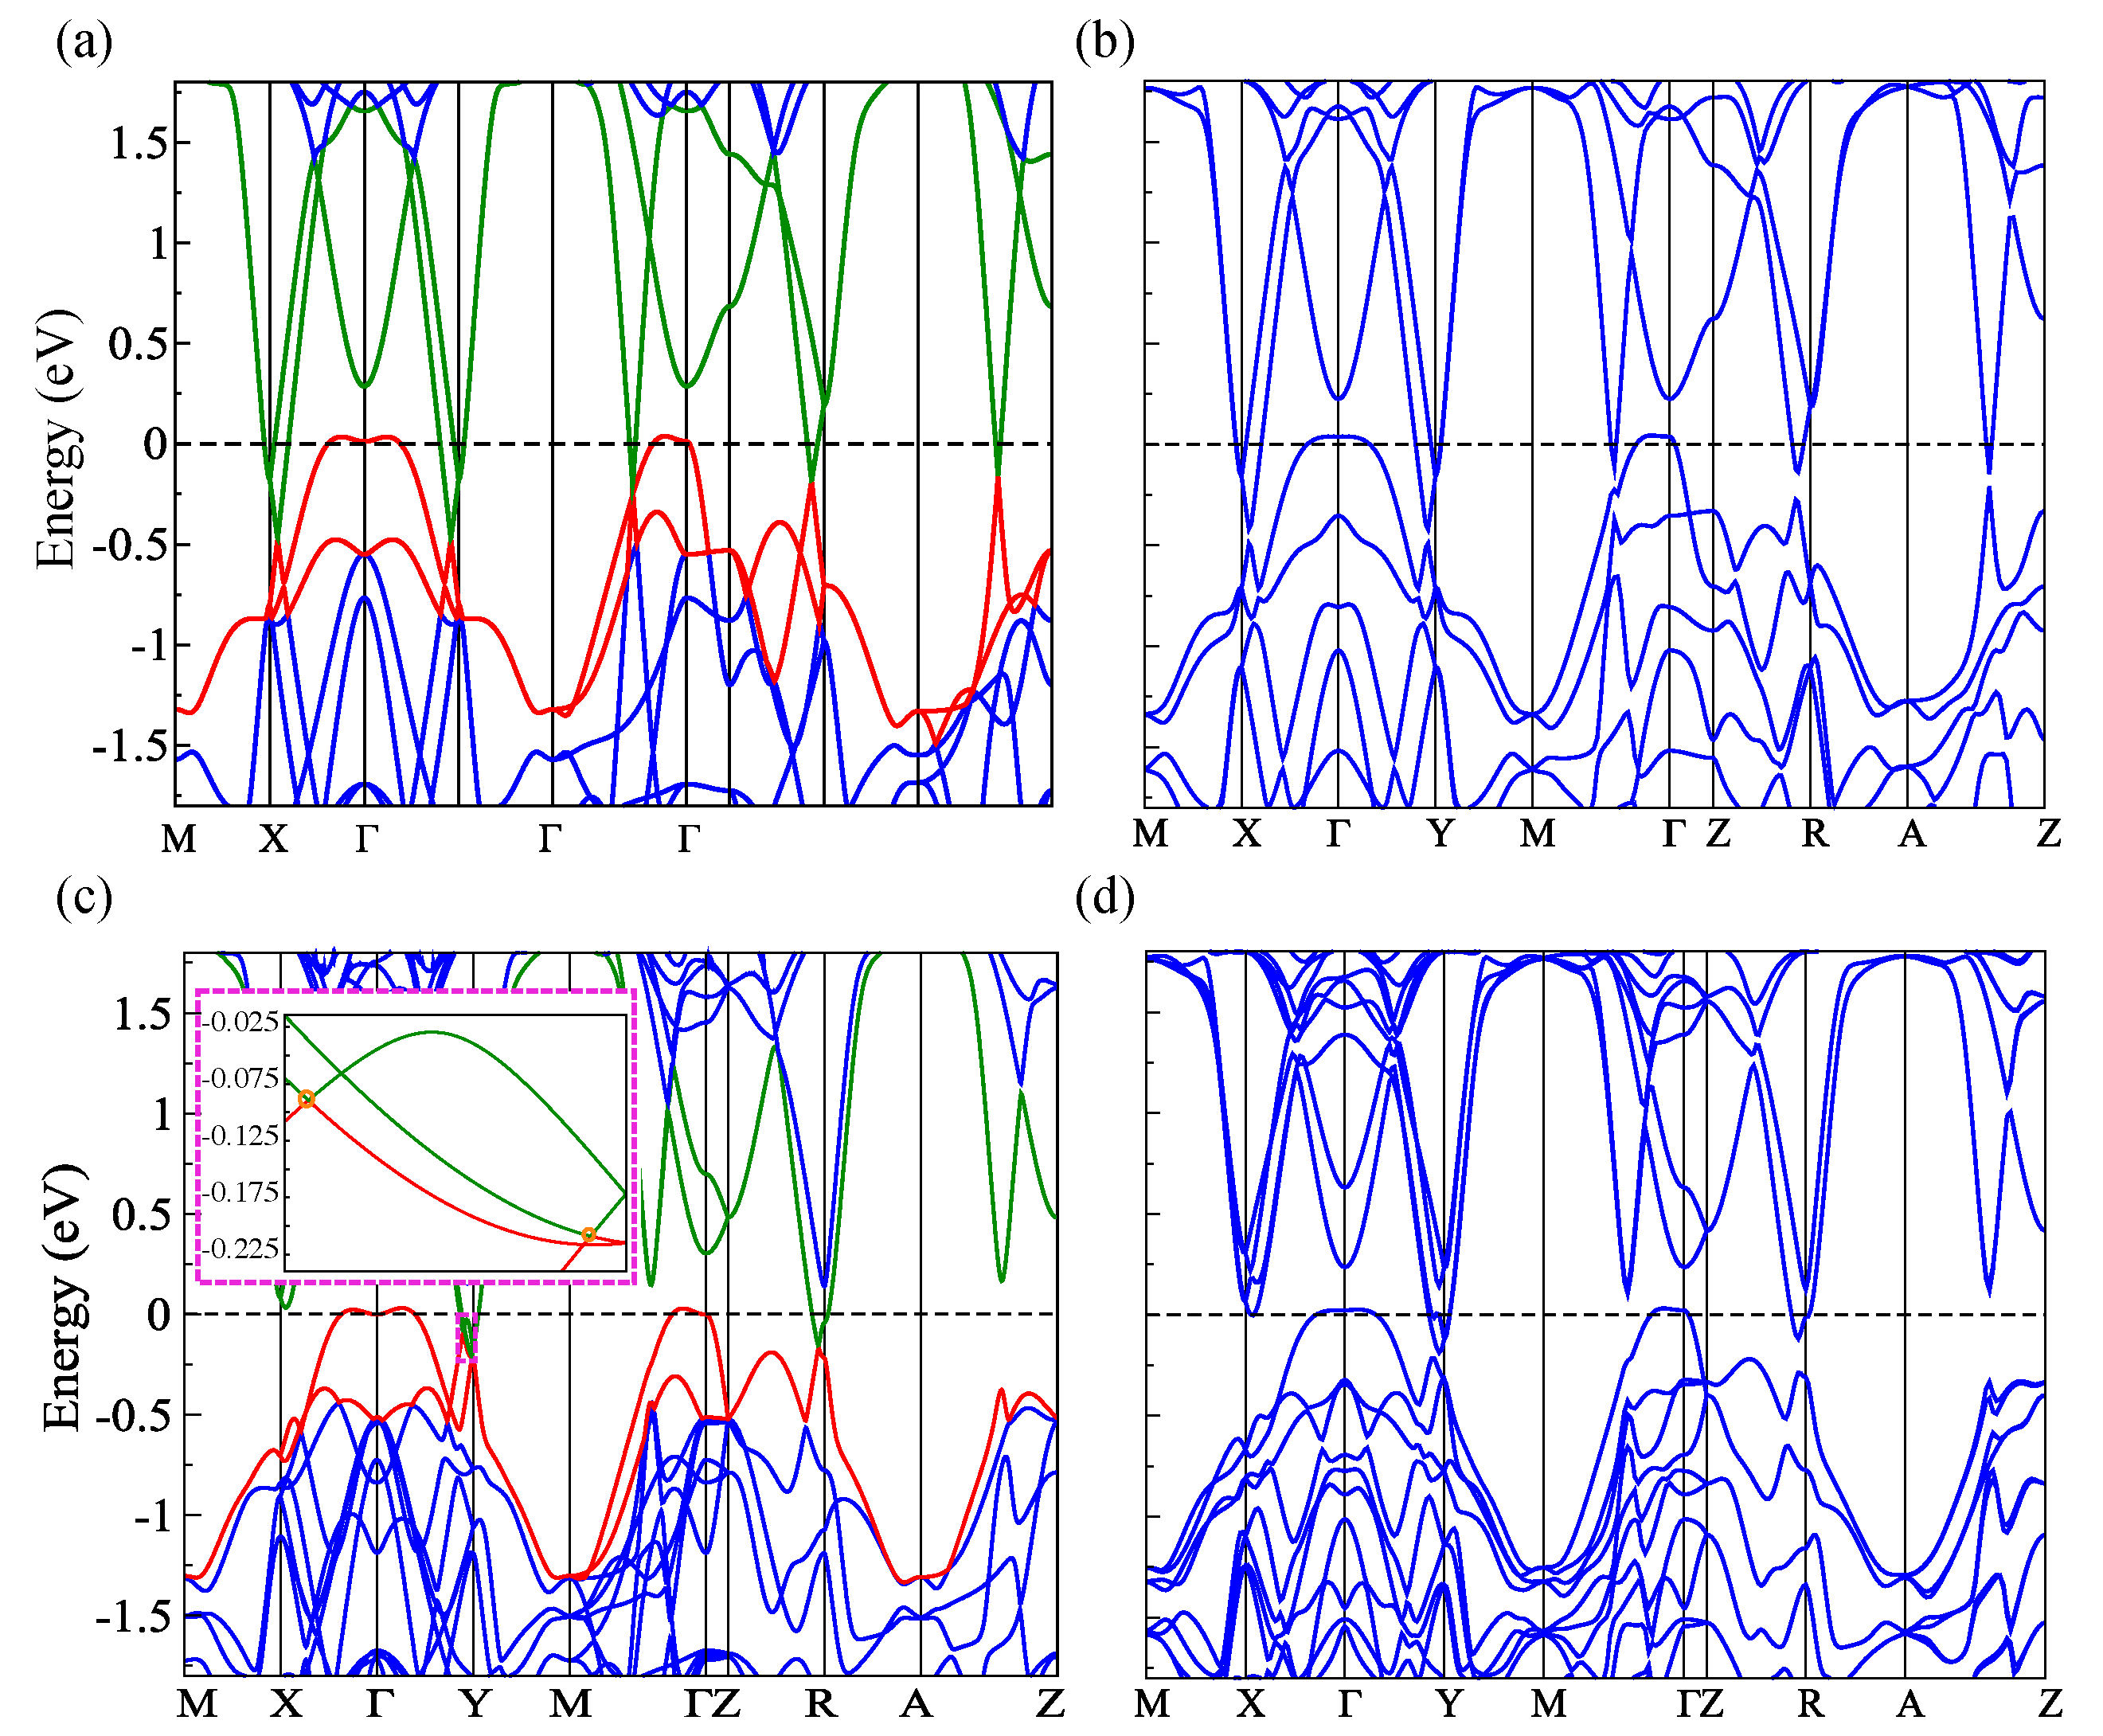
\includegraphics[width=1\textwidth]{lasbte-fig3.pdf}
    \bicaption{
    对 \ti~(a,c)和~\tci~(b,d)用GGA不考虑(a,b)和考虑(c,d)SOC时,沿着高对称线计算的能带结构。图(c)中的插图展示了不考虑SOC时沿着$\Gamma-$Y的能带反转。两条最高的价带和两条最低的导带分别用红色和绿色标记。~\citep{qian2020layer}
    }
    {
        Calculated band structures along the high-symmetry lines within GGA without (a, c) and with (b, d) SOC for~\ti~(a, b) and \tci~(c, d). The inset in (c) shows the band inversion feature along $\Gamma-$Y without SOC for \tci. The two highest valance bands and lowest conduction bands are marked in red and green, respectively. ~\citep{qian2020layer}
    }
    \label{fig:3-2}
\end{figure}
%figure

\ti~和~\tci~考虑和不考虑SOC的能带结构如图~\ref{fig:3-2}所示。众所周知,作为$WHM$家族的材料之一,在SOC忽略的情况下,\ti~有节点线结构~\citep{xu2015two, lou2016emergence}。 显而易见,在$k_z=0$的平面,沿着$\Gamma-X (Y)$和 $\Gamma-M$路径,在$k_z=\pi$平面,沿着$Z-R$,$Z-A$路径有能带交叉点。当SOC考虑进来时,所有节点线都打开带隙,从而使得\ti~成为弱拓扑绝缘体,按照QLs,即2维拓扑绝缘体的简单堆叠~\citep{xu2015two}。在不考虑SOC时,\tci~的能带结构也有交叉点,这些交点实际上是镜面$m^{100}_{\frac{1}{2}00 }$上节点线的一部分,如图\ref{fig:3-1}(f)所示。同时,SOC将使得节点线打开能隙,但会使得\tci~成为拓扑晶体绝缘体。


根据对称指标理论~\citep{nc_ashvin,wanxg2019},\ti~和~\tci~都有中心反演对称性,而且当考虑SOC时,他们的对称性指标为$\mathbb Z_{2,2,2,4}$,这个可以简单地通过类Fu-Kane公式得到~\citep{song2017, prx_ashvin}。三个弱拓扑指标$\mathbb Z_2$,标记为$z_{2w,i=1,2,3}$可以由以下公式计算得到:
%%equation%%%
\begin{equation}
\label{eq:1}
\begin{aligned}
z_{2w,i=1,2,3}\equiv&\sum_{\rm {\bold K}\in TRIM \;at \;\{k_i=\pi\}} n^{-}_{\bold K} \; \mathrm {mod} \;{2}
\end{aligned} .
\end{equation}
%%equation%%%

$\mathbb Z_4$指标记作$z_4$可由:
%%equation%%%
\begin{equation}
\label{eq:2}
\begin{aligned}
 z_4  \equiv \sum_{\rm \bold K \in TRIM} \frac {n^{-}_{\bold K} -n^{+}_{\bold K}}{2}  \; \mathrm {mod} \;{4}
 \end{aligned} ,
\end{equation}
%%equation%%%
获得,这里$n^{+}_{\bold K}$ ($n^{-}_{\bold K}$) 是时间反演不变点$\bold K$上占据态克拉默对有宇称为$+(-)$的数目。占据态克拉默对有宇称为负的数目已经在图~\ref{fig:3-1}中标出。 因此,根据方程~\ref{eq:1}和方程~\ref{eq:2},我们可以知道~\ti~有拓扑指标$\mathbb Z_{2,2,2,4}$为(0010)的弱拓扑绝缘体,而~\tci~是有拓扑指标为(0002)的拓扑绝缘体。我们知道每个单层,即~\ti~的QL是一个二维拓扑绝缘体~\citep{xu2015two}。在相变之后,形变的QL仍然是二维的拓扑绝缘体。在~\tci~原胞内是两个弱耦合的QLs的简单堆叠。这些不同之处和他们相应的拓扑不变量以及拓扑性质可以进一步通过层构造方案来理解,这个方法可以将实空间的晶体结构与倒空间能带拓扑联系起来。

\subsection{层构造和拓扑不变量}
直观上,\ti~可以看成是通过在密勒指数为(001; $\frac{1}{2}$)的平面上放置一层二维拓扑绝缘体来构造的。应用129号空间群所有的对称操作只能给出同样的密勒面。因此基本层构造eLC (001; $\frac{1}{2}$) 如图~\ref{fig:3-1} (b) 所示。在每个原胞内,这个eLC与$a$轴和$b$轴相交零次,和$c$轴相交一次,给出三个弱拓扑不变量$z_{2w, i=1, 2, 3}=0,0,1$。eLC (001; $\frac{1}{2}$) 占据8个反演中心中的四个,这意味着对于这个eLC由中心反演对称性保护的拓扑不变量$\delta_i$是规范依赖的,所以$z_4=0$, $\delta_i=0$。这个eLC不占据任何旋转轴,螺旋轴,镜面或者滑移面。并且,对于螺旋和滑移操作,它不给出任何非零的堆叠不变量。这意味旋转,螺旋,镜面和滑移所对应的拓扑不变量都是零,因此~\ti~是弱拓扑绝缘体而不是拓扑晶体绝缘体。

从~\ti~到~\tci~的结构相变已经通过~\ti~在$Z$点的软模表明。这导致结构沿着$c$轴的加倍和原子的移动。因此在~\tci~的原胞有两个二维拓扑绝缘体,位于密勒面 (001; $\frac{1}{4}$) 和 (001; $\frac{3}{4}$) 。这两个二维拓扑绝缘体构成62号群的一个eLC (001; $\frac{1}{4}$) 或者eLC  (001; $\frac{3}{4}$) 。在本文所选择的规范下,这两个层与三个晶格矢量相交偶数次,所以$z_{2w, i=1, 2, 3}=0$。在图~\ref{fig:3-1} (e) 中所有的反演中心都被这两个二维拓扑绝缘体占据了, 这表明$\delta_i=1$,$z_4=2$。同样地,这个eLC不占据任何镜面和滑移面,也不穿过任何旋转轴。但是,滑移面 $g^{010}_{0\frac{1}{2}\frac{1}{2}}$和螺旋轴 $2^{100}_{ \frac{1}{2}0\frac{1}{2}}$,$2^{001}_{\frac{1}{2}\frac{1}{2}\frac{1}{2}}$会贡献非零的堆叠不变量。所以,相应的拓扑滑移不变量$\delta_h$和螺旋不变量$\delta_s$等于1。通过这个方法,~\tci~的时间反演对称和晶体对称性所保护的拓扑态都被完全确定下来了。它是一个拓扑晶体绝缘体,相应的对称性指标为$\mathbb Z_{2,2,2,4}=(0002)$,拓扑不变量为  $\delta_i=1$, $\delta_{h}^{(010)}=1$和$\delta_{s}^{(100)}=\delta_{s}^{(001)}=1$。
 

\subsection{从拓扑不变量到拓扑表面态}

\begin{figure*}[!htb]
\centering
\includegraphics[width=15 cm]{lasbte-fig4.pdf}
\bicaption{
在(100)(a-c)和(1$\bar 1$0)(d-f)表面的Wilson loop谱和表面态能带结构。(b, e)分别是(a)和(d)阴影部分的放大。可以很清楚的看到在(b,c)中有沙漏型的拓扑表面态,但是(e, f)中有开能隙的平庸的表面态。~\citep{qian2020layer}
}
{
The spectra of Wilson loop and SS band structures on surface BZ of (100) (a-c) and (1$\bar 1$0) (d-f) surfaces, respectively. (b, e) The zoomed in image of the shadowed part in (a) and (d), respectively. It can be seen clearly that there are hourglass-like SSs in (b, c) but trivial SSs with full gap in (e, f). ~\citep{qian2020layer}
}
\label{fig:3-4}
\end{figure*}

不平庸的滑移不变量$\delta_h$表明存在不平庸的沙漏型拓扑表面态在保持相应的滑移对称性的表面上~\citep{wang2016hourglass,bernevigprx}。
我们知道,定义在布里渊区占据态纤维丛上的Wilson loop谱同构于表面态能谱~\citep{fidkowski2011model}。我们可以通过计算体态哈密顿量Wilson loop谱或者计算截断表面作为边界条件的表面格林函数得到表面态,来验证滑移不变量的正确性。~\citep{WU2017,Sancho_1985}。
在(100)表面,由于滑移对称性$g^{010}_{0\frac{1}{2}\frac{1}{2}}$保持并且投影到$\bar\Gamma-\bar Z$和$\bar R-\bar Y$路径,滑移不变量$\delta_{h}^{(010)}=1$可以保护不平庸的沙漏型表面存在,如图~\ref{fig:3-1}(f)所示。
在~\ref{fig:3-4} (a)和(b)中,Wilson loop谱清楚地显示$\bar\Gamma-\bar Z$ and $\bar R-\bar Y$有沙漏型的表面态。而且两个沙漏型表面态之间$\bar Z-\bar R$路径的连接曲线有一般的锯齿形图案,表现出谱状结构~\citep{bernevigprx}。通过格林函数方法计算表面态,我们发现沿着$\bar\Gamma-\bar Z$路径可以清晰地看到沙漏型的表面态,如图~\ref{fig:3-4}(c)所示。但是,沿着$\bar R-\bar Y$的表面态由于混合到体态中很难被看到。
类似地,不变量$\delta_{h}^{(001)}$是平庸的,所以在(1$\bar1$0)表面,当投影到$\tilde Z-\tilde R$和$\tilde Y-\tilde\Gamma$方向(保持$g^{001}_{\frac{1}{2} \frac{1}{2} 0 }$对称性)时,应该有平庸的表面态。
在图~\ref{fig:3-4}(d, e)中沿着$\tilde Z-\tilde R$ 和 $\tilde Y-\tilde\Gamma$方向,沙漏型的表面态其实是平庸的。因为当在整个表面布里渊区沿着$\tilde Z\tilde R\tilde Y\tilde\Gamma$看,他们之间的连接方式在谱线上有明显的能隙,表现出各自孤立的状态,这和图~\ref{fig:3-4}(f)中拓扑平庸的表面态计算结果相吻合。

不平庸的滑移不变量$\delta_s$可以保护棱态,这些已经在很多工作中~\citep{wang2016hourglass,Fangc2t,zhangt2019}被详细讨论过,在此为了简洁起见将不再赘述。


\section{结论}
基于第一性原理计算,我们发现拓扑晶体绝缘体相\tci~有沙漏型的表面态和棱态,可以看作是两个\ti~由于结构相变而来。这种维度降低的方法可以有效的抓住拓扑晶体绝缘体的物理本质。 
特别是据我们所知道,这是第一次找到一个实验可以得到的材料能够生动形象地将实空间的层构造和动量空间的能带拓扑相对应。例如对于拓扑晶体绝缘体家族 Ba$_3$Cd$_2$As$_4$ \citep{zhangt2019}也可以看作是由层构造: $(001;0){\otimes} (001;\frac{1}{2})$得到,但是这个层构造不能直接对应于实空间的晶体结构。所以这个完美的例子为我们理解拓扑晶体绝缘体和拓扑绝缘体的关系和物理本质提供了非常好的平台。